

\section{Prueba 6}
\subsection{Red de inferencia}
\begin{center}
	\tikzstyle{regla}= [rectangle,draw,black,fill=blue!15]
	\tikzstyle{hecho}= [rectangle,draw,black,fill=black!15]
	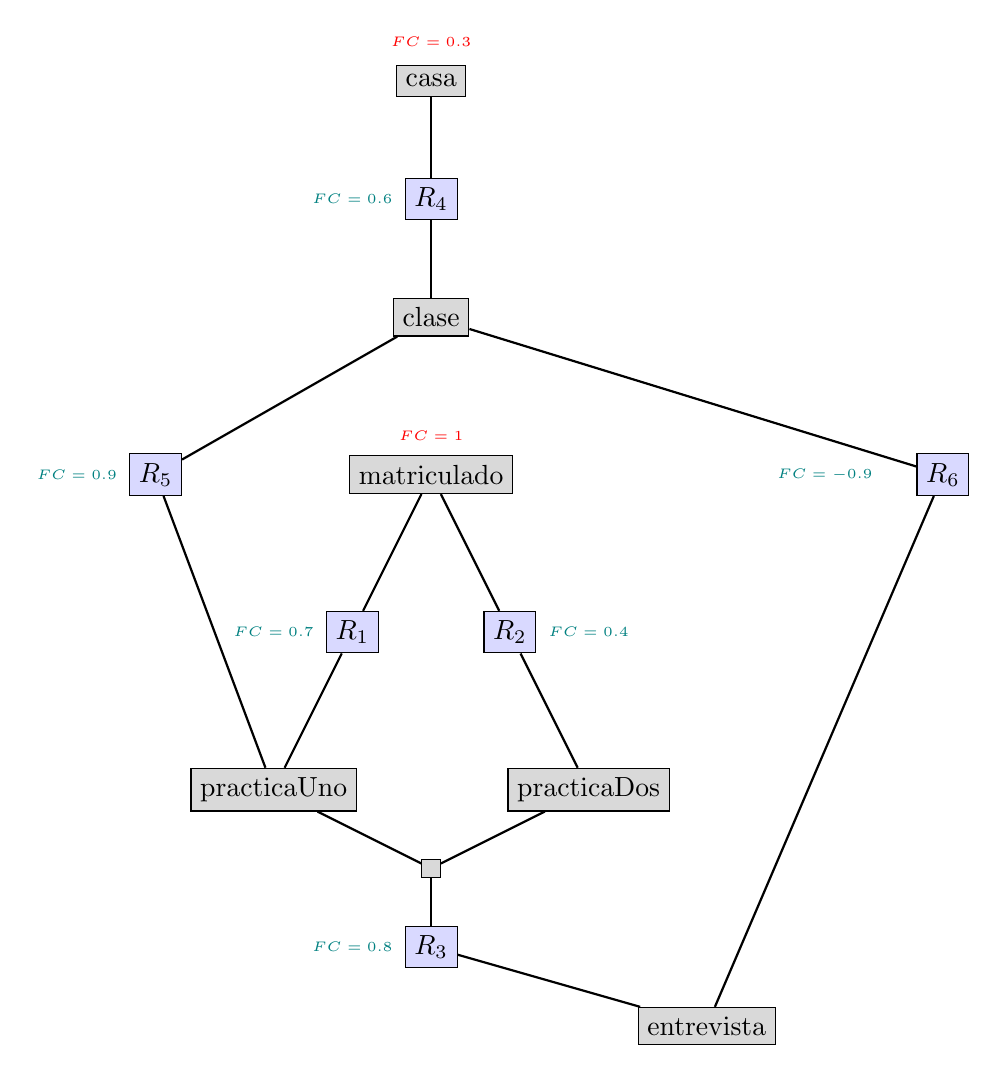
\begin{tikzpicture}
		
		\node (a) at (1,5) [hecho] {casa};
		\node at (1,5.5) {\color{red}{\tiny{$FC=0.3$}}};

		\node (b) at (1,2) [hecho] {clase};

		\node (c) at (1,0) [hecho] {matriculado};
		\node at (1,0.5) {\color{red}{\tiny{$FC=1$}}};

		\node (d) at (-1,-4)[hecho] {practicaUno};

		\node (e) at (3,-4)[hecho] {practicaDos};
		
		\node (f) at (4.5,-7)[hecho] {entrevista};

		\node (d/e) at (1,-5)[hecho] {};

		\node (r1) at (0,-2) [regla] {$R_{1}$};
		\node at (-1,-2) {\color{teal}{\tiny{$FC=0.7$}}};
		\node (r2) at (2,-2) [regla] {$R_{2}$};
		\node at (3,-2) {\color{teal}{\tiny{$FC=0.4$}}};
		\node (r3) at (1,-6) [regla] {$R_{3}$};
		\node at (0,-6) {\color{teal}{\tiny{$FC=0.8$}}};
		\node (r4) at (1,3.5) [regla] {$R_{4}$};
		\node at (0,3.5) {\color{teal}{\tiny{$FC=0.6$}}};
		\node (r5) at (-2.5,0) [regla] {$R_{5}$};
		\node at (-3.5,0) {\color{teal}{\tiny{$FC=0.9$}}};
		\node (r6) at (7.5,0) [regla] {$R_{6}$};
		\node at (6,0) {\color{teal}{\tiny{$FC=-0.9$}}};
		
		\path[black,thick] (a) edge[] node {} (r4);
		\path[black,thick] (r4) edge[] node {} (b);
		\path[black,thick] (b) edge[] node {} (r5);
		\path[black,thick] (r5) edge[] node {} (d);
		\path[black,thick] (b) edge[] node {} (r6);
		\path[black,thick] (r6) edge[] node {} (f);

        \path[black,thick] (c) edge[] node {} (r1);
		\path[black,thick] (r1) edge[] node {} (d);
		\path[black,thick] (d) edge[] node {} (d/e);
		\path[black,thick] (c) edge[] node {} (r2);
		\path[black,thick] (r2) edge[] node {} (e);
		\path[black,thick] (e) edge[] node {} (d/e);
		\path[black,thick] (d/e) edge[] node {} (r3);
		\path[black,thick] (r3) edge[] node {} (f);


	\end{tikzpicture}
\end{center}
\par Esta red de inferencia se debe interpretar de arriba a abajo.
Los rectángulos azules son las reglas, los grises que están ligados por encima 
de ellas son sus antecedentes, si estos antecedentes convergen en un cuadrado 
quiere decir que es la conjunción de esos literales, en caso contrario son disyunciones
o simplemente un literal. Los rectángulos grises que cuelgan de las reglas 
son sus consecuentes respectivamente. Además, incluyo los factores de certeza propocionados por
la Base de hechos y la Base de Conocimiento iniciales.

\subsection{Proceso de inferencia}
\begin{listing}[language=Pascal]
(Razonamiento dirigido por Metas)
Objetivo: entrevista
Proceso de Inferencia: 
  ###########################
  # Llamada (1) a verificar #
  ###########################
	Verificar(entrevista,{casa,matriculado}) // Recursion 
	Conjunto Conflicto={R3,R6} // entrevista es consecuente de estas reglas
	R={R3} // Seleccionar regla R3
	Eliminar R3 ---> Conjunto Conflicto={R6}
	NuevasMetas={practicaDos,practicaUno} // Antecedentes de R3; Verificado = true
	Meta=practicaDos // Seleccionar practicaDos de NuevasMetas
	NuevasMetas={practicaUno} // Eliminar practicaDos de NuevasMetas
  ###########################
  # Llamada (2) a verificar #
  ###########################
	Verificar(practicaDos,{casa,matriculado}) // Recursion 
	Conjunto Conflicto={R2} // practicaDos es consecuente de estas reglas
	R={R2} // Seleccionar regla R2
	Eliminar R2 ---> Conjunto Conflicto={}
	NuevasMetas={matriculado} // Antecedentes de R2; Verificado = true
	Meta=matriculado // Seleccionar matriculado de NuevasMetas
	NuevasMetas={} // Eliminar matriculado de NuevasMetas
  ###########################
  # Llamada (3) a verificar #
  ###########################
	Verificar(matriculado,{casa,matriculado}) ---> true // Recursion: matriculado en BH
	BH={casa,matriculado}
	(CASO 3): Combinacion de la evidencia con la regla R2
	 FC(practicaDos{R2})=0.4*max(0,FC(matriculado))=0.4
	BH={casa,matriculado,practicaDos} // Insertar practicaDos a la Base de Hechos
	Meta=practicaUno // Seleccionar practicaUno de NuevasMetas
	NuevasMetas={} // Eliminar practicaUno de NuevasMetas
  ###########################
  # Llamada (4) a verificar #
  ###########################
	Verificar(practicaUno,{casa,matriculado,practicaDos}) // Recursion 
	Conjunto Conflicto={R1,R5} // practicaUno es consecuente de estas reglas
	R={R1} // Seleccionar regla R1
	Eliminar R1 ---> Conjunto Conflicto={R5}
	NuevasMetas={matriculado} // Antecedentes de R1; Verificado = true
	Meta=matriculado // Seleccionar matriculado de NuevasMetas
	NuevasMetas={} // Eliminar matriculado de NuevasMetas
  ###########################
  # Llamada (5) a verificar #
  ########################
	Verificar(matriculado,{casa,matriculado,practicaDos}) ---> true // Recursion: matriculado en BH
	BH={casa,matriculado,practicaDos}
	(CASO 3): Combinacion de la evidencia con la regla R1
	 FC(practicaUno{R1})=0.7*max(0,FC(matriculado))=0.7
	Conjunto Conflicto={R5} // practicaUno es consecuente de estas reglas
	R={R5} // Seleccionar regla R5
	Eliminar R5 ---> Conjunto Conflicto={}
	NuevasMetas={clase} // Antecedentes de R5; Verificado = true
	Meta=clase // Seleccionar clase de NuevasMetas
	NuevasMetas={} // Eliminar clase de NuevasMetas
  ###########################
  # Llamada (6) a verificar #
  ###########################
	Verificar(clase,{casa,matriculado,practicaDos}) // Recursion 
	Conjunto Conflicto={R4} // clase es consecuente de estas reglas
	R={R4} // Seleccionar regla R4
	Eliminar R4 ---> Conjunto Conflicto={}
	NuevasMetas={casa} // Antecedentes de R4; Verificado = true
	Meta=casa // Seleccionar casa de NuevasMetas
	NuevasMetas={} // Eliminar casa de NuevasMetas
  ###########################
  # Llamada (7) a verificar #
  ###########################
	Verificar(casa,{casa,matriculado,practicaDos}) ---> true // Recursion: casa en BH
	BH={casa,matriculado,practicaDos}
	(CASO 3): Combinacion de la evidencia con la regla R4
	 FC(clase{R4})=0.6*max(0,FC(casa))=0.18
	BH={casa,clase,matriculado,practicaDos} // Insertar clase a la Base de Hechos
	(CASO 3): Combinacion de la evidencia con la regla R5
	 FC(practicaUno{R5})=0.9*max(0,FC(clase))=0.162
	(CASO 2): Combinacion de las reglas R1 y R5
	 FC(practicaUno)=FC(practicaUno{R1}) + FC(practicaUno{R5})*(1-FC(practicaUno{R1}))=0.7486
	BH={casa,clase,matriculado,practicaDos,practicaUno} // Insertar practicaUno a la Base de Hechos
	(CASO 1): Combinacion de antecedentes de R3
	 FC(practicaUno y practicaDos)= min(FC(practicaDos),FC(practicaUno))=0.4
	(CASO 3): Combinacion de la evidencia con la regla R3
	 FC(entrevista{R3})=0.8*max(0,FC(practicaUno y practicaDos))=0.32
	Conjunto Conflicto={R6} // entrevista es consecuente de estas reglas
	R={R6} // Seleccionar regla R6
	Eliminar R6 ---> Conjunto Conflicto={}
	NuevasMetas={clase} // Antecedentes de R6; Verificado = true
	Meta=clase // Seleccionar clase de NuevasMetas
	NuevasMetas={} // Eliminar clase de NuevasMetas
  ###########################
  # Llamada (8) a verificar #
  ###########################
	Verificar(clase,{casa,clase,matriculado,practicaDos,
	practicaUno}) ---> true // Recursion: clase en BH
	BH={casa,clase,matriculado,practicaDos,practicaUno}
	(CASO 3): Combinacion de la evidencia con la regla R6
	 FC(entrevista{R6})=-0.9*max(0,FC(clase))=-0.162
	(CASO 2): Combinacion de las reglas R3 y R6
	 FC(entrevista)=FC(entrevista{R3}) + FC(entrevista{R6})/(1-min{|FC(entrevista{R3}|), FC(entrevista{R3}|})=0.188544
	BH={casa,clase,entrevista,matriculado,practicaDos,
	practicaUno} // Insertar entrevista a la Base de Hechos
Return TRUE
\end{listing}

\subsection{Objetivo obtenido por SBR-FC}
\begin{center}
\par -------------------- Hecho (entrevista) ---------------------
\par Hecho (nomHecho): entrevista
\par Hecho (facCerBH): 0.188544
\par ------------------------------------------------------------
\end{center}
